\documentclass[11pt,a4paper,twoside,openright]{book} %report

\usepackage{url,amsfonts,epsfig}
\usepackage{afterpage}
\usepackage{amsmath,amssymb}            
\usepackage{rotating}  
\usepackage{fancyhdr}  
%\usepackage[scriptsize]{caption2} 
%\hyphenation{a-gen-tiz-za-zio-ne}

%\setlength{\paperwidth}{16cm}
%\setlength{\paperheight}{24cm}
%\setlength{\oddsidemargin} {2. cm}
%\setlength{\evensidemargin} {2. cm}
\addtolength{\oddsidemargin} {-0.4 cm}
\addtolength{\evensidemargin} {-0.4 cm}
\linespread{1.1}
\usepackage[italian]{babel}
%\usepackage[latin1]{inputenc}
%\renewcommand{\captionfont}{\normalfont \sffamily \itshape \small}

\pagestyle{empty}

\usepackage{graphicx}
\graphicspath{ {images/} }

\title{Esame di Elementi di Data Mining}
\author{Filippo Bisconcin, 852144}
\date{28 Maggio 2018}

\begin{document}

\frontmatter

\thispagestyle{empty}
%\begin{titlepage}
\vspace*{-1.5cm}


\includegraphics[height=4.5cm]{images/unive.pdf}

\begin{center}

\vspace*{1.0cm}

\LARGE
Corso di Laurea in Informatica

\vspace*{2.0cm}

Analisi dello Stato Italiano

\vspace*{1.0cm}

\begin{large}
\textbf{Esame di Elementi di Data Mining}
\end{large}

\end{center}

\vspace*{2.5cm}

\begin{flushleft}

\textbf{Studente}

Filippo Bisconcin, 852144

\vspace*{1.0cm}

\textbf{Anno Accademico}

2017-2018
\end{flushleft}


%\thispagestyle{empty} \normalfont \cleardoublepage

%\thispagestyle{empty} \vspace*{.75truecm} \normalfont \cleardoublepage


\pagestyle{plain}
\tableofcontents
\pagestyle{empty}\cleardoublepage
\pagenumbering{arabic}

\pagestyle{fancy} 
\fancyfoot{}                                               
\renewcommand{\chaptermark}[1]{\markboth{\chaptername\ \thechapter.\ #1}{}} 
\renewcommand{\sectionmark}[1]{\markright{\thesection.\ #1}}         
\fancyhead[LE,RO]{\bfseries\thepage}    
                                        
\fancyhead[RE]{\bfseries\leftmark}    
\fancyhead[LO]{\bfseries\rightmark}     
\renewcommand{\headrulewidth}{0.3pt} 

Con la presente ricerca vorrei analizzare alcuni dataset riguardanti vari aspetti dello Stato Italiano.

I dataset utilizzati sono stati generati da indagini svolte in diversi periodi.




\mainmatter

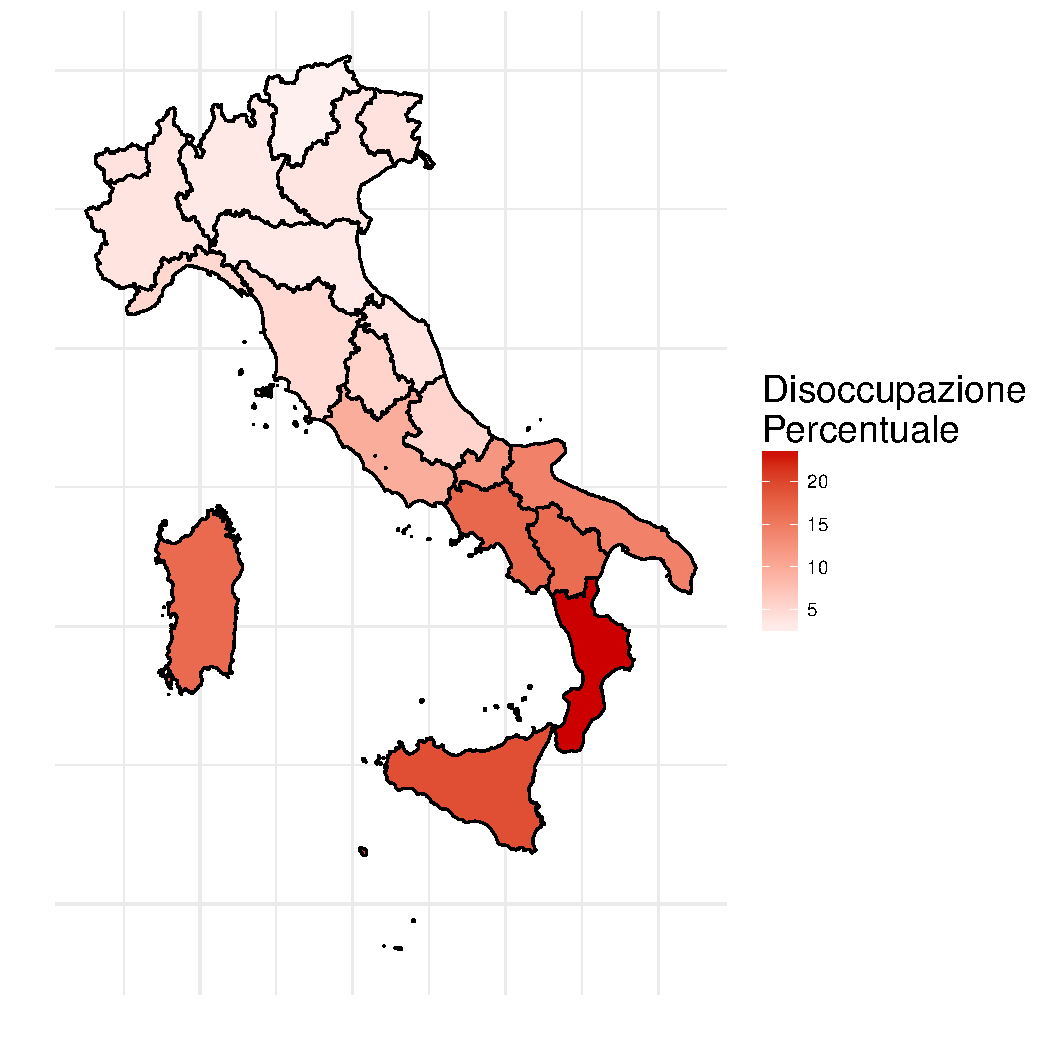
\includegraphics[height=10cm]{disoccupazione_percentuale.pdf}


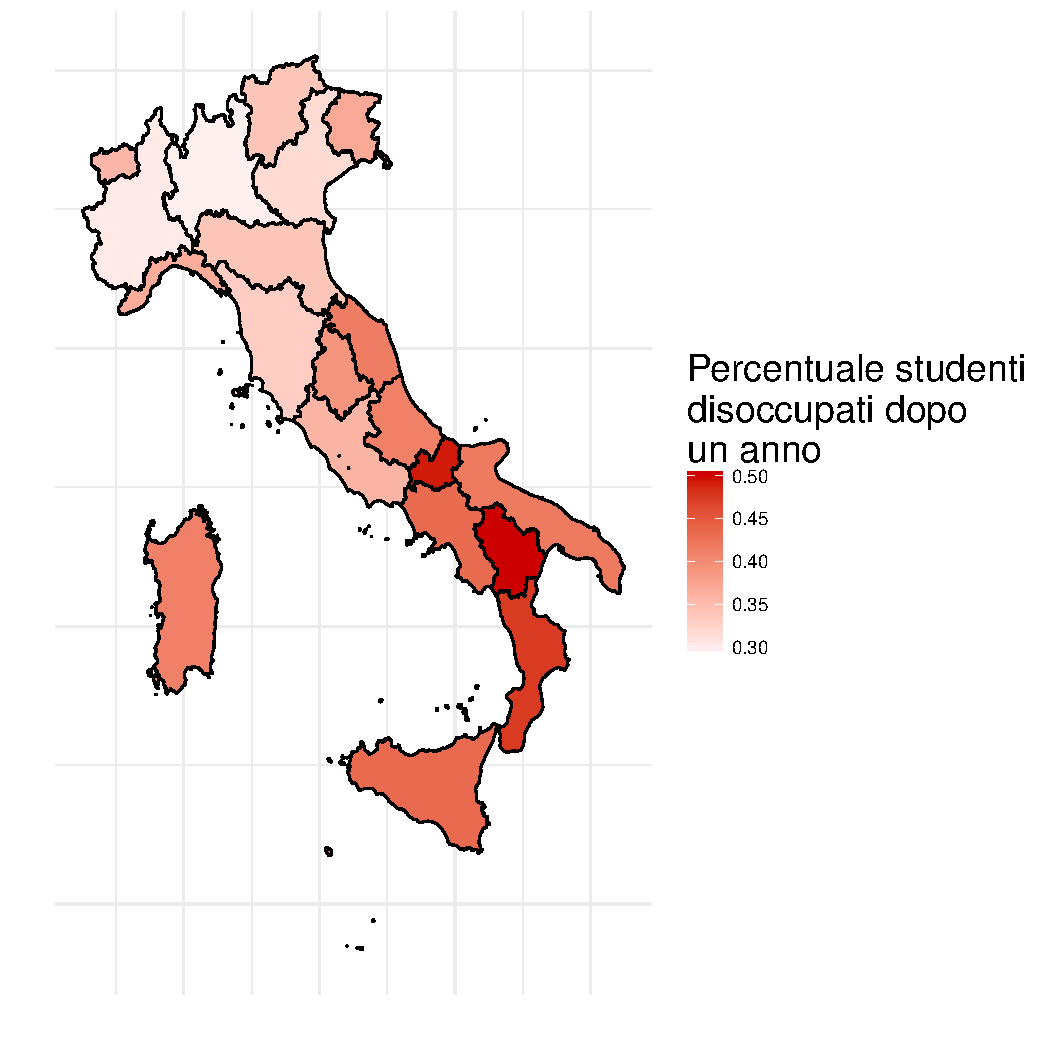
\includegraphics[height=10cm]{occupazione_post_laurea.pdf}


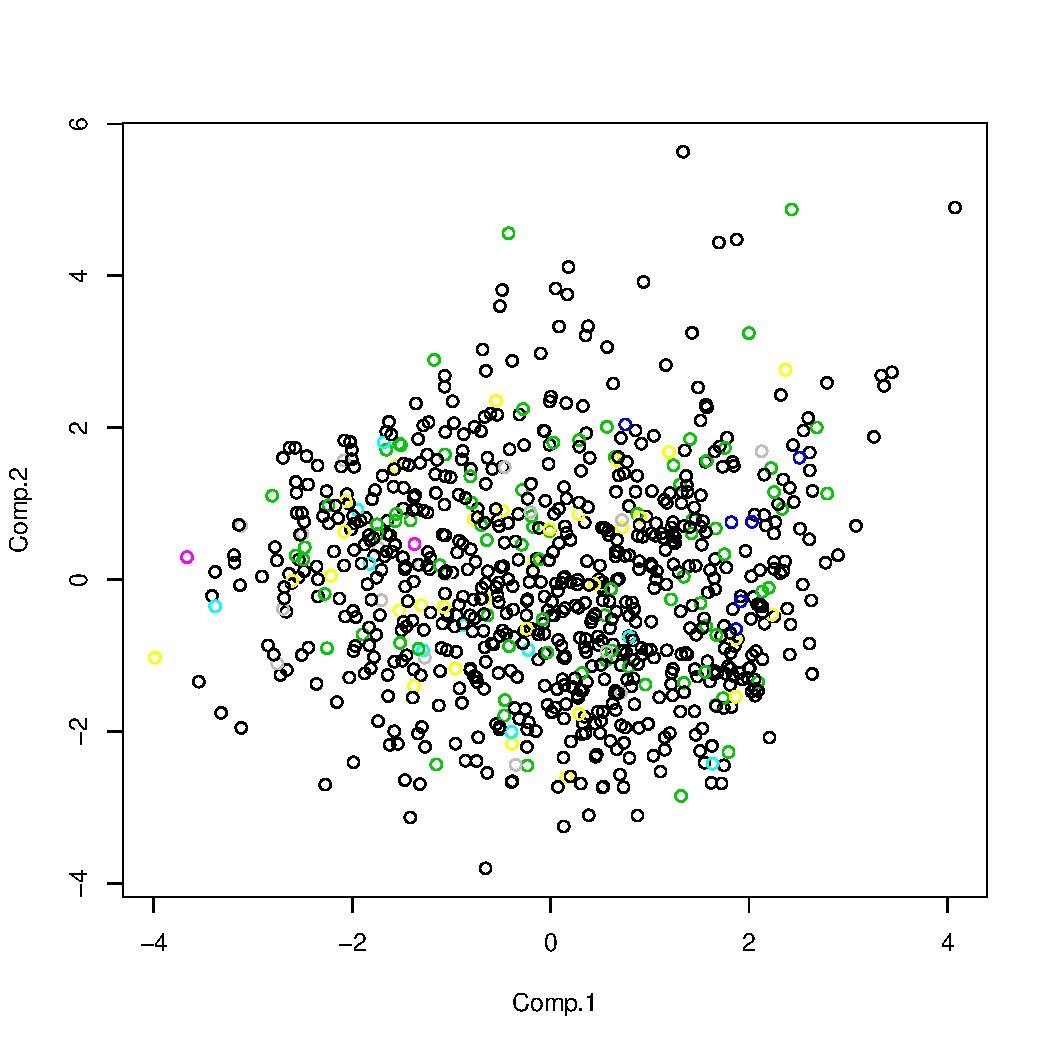
\includegraphics[height=10cm]{pc_1_2.pdf}

\backmatter

\end{document}